
\parbox[t]{8cm}{\medskip
	\emph{Dans cet exercice, aucune justification n'est attendue}
	
\bigskip
	
On considère l'hexagone ABCDEF de centre O représenté ci-contre.}
\hfill 
\begin{tikzpicture}[x=25mm,y=25mm,baseline={(A)},,line width=1pt]
\newcommand{\point}[3]{\draw[shift={#1}] (-3pt,-3pt)--(3pt,3pt) (-3pt,3pt)--(3pt,-3pt) (0,0) node[shift={#2}]{#3};}
	
\coordinate (A) at (120:1); \point{(A)}{(120:3mm)}{A};
\coordinate (B) at ( 60:1); \point{(B)}{( 60:3mm)}{B};
\coordinate (C) at (  0:1); \point{(C)}{(  0:3mm)}{C};
\coordinate (D) at (300:1); \point{(D)}{(300:3mm)}{D};
\coordinate (E) at (240:1); \point{(E)}{(240:3mm)}{E};
\coordinate (F) at (180:1); \point{(F)}{(180:3mm)}{F};
\coordinate (O) at (0 , 0); \point{(O)}{(270:3mm)}{O};

\draw (A)--(B) node[pos=0.5,sloped]{||}
	--(C) node[pos=0.5,sloped]{||}
	--(D) node[pos=0.5,sloped]{||}
	--(E) node[pos=0.5,sloped]{||}
	--(F) node[pos=0.5,sloped]{||}
	--cycle node[pos=0.5,sloped]{||}
	(A)--(O) node[pos=0.5,sloped]{||}
	(B)--(O) node[pos=0.5,sloped]{||}
	(C)--(O) node[pos=0.5,sloped]{||}
	(D)--(O) node[pos=0.5,sloped]{||}
	(E)--(O) node[pos=0.5,sloped]{||}
	(F)--(O) node[pos=0.5,sloped]{||};
	\end{tikzpicture}

\begin{enumerate}
	\item  Parmi les propositions suivantes, recopier celle qui correspond à l'image du quadrilatère CDEO par la symétrie de centre O.
	
\renewcommand{\arraystretch}{1.5}
\begin{tabularx}{\linewidth}{|*{3}{>{\centering \arraybackslash} X|}} \hline
		\textbf{Proposition 1}&\textbf{Proposition 2}&\textbf{Proposition 3}\\ \hline
		FABO & ABCO & FODE\\ \hline
	\end{tabularx}
		
		\item Quelle est l'image du segment [AO] par la symétrie d'axe (CF) ?
		
		\item  On considère la rotation de centre O qui transforme le triangle OAB en le triangle OCD.
		
		Quelle est l'image du triangle BOC par cette rotation ?
	\end{enumerate}
\parbox{8cm}{La figure ci-contre représente un pavage dont le motif de base a la même forme que l'hexagone ci-dessus.
On a numéroté certains de ces hexagones.
	\begin{enumerate}[start=4]
		\item Quelle est l'image de l'hexagone 14 par la translation qui transforme l'hexagone 2 en l'hexagone 12 ?
\end{enumerate}}\hfill 
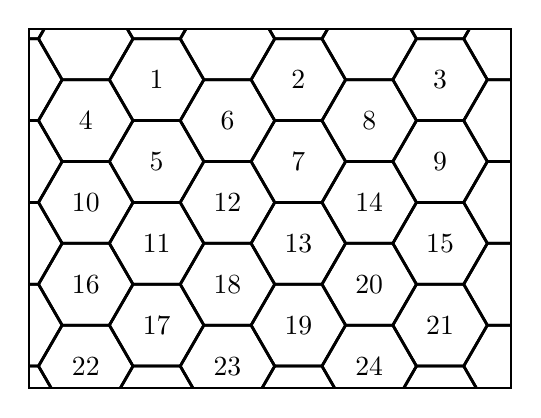
\begin{tikzpicture}[x=0.6cm,y=0.6cm,line width=1pt,baseline={(current bounding box.center)}]
%\draw[teal,xstep=1,ystep=1] (0,0) grid (10,10);
\clip[draw] (0.3,0.4) rectangle (10.5,8);
\foreach \x  in {0,...,3}{
\foreach \y in {0,...,5}
\draw[shift={({3*\x},{1.732*\y})}] (0:1)--(60:1)--(120:1)--(180:1)--(240:1)--(300:1)--cycle (0,0);}
\foreach \x  in {0,...,3}{
\foreach \y in {0,...,5}
\draw[shift={({1.5+3*\x},{0.866+1.732*\y})}] (0:1)--(60:1)--(120:1)--(180:1)--(240:1)--(300:1)--cycle;}
\node at(3,6.928) {1}; \node at(6,6.928) {2}; \node at(9,6.928) {3};
\node at(3,5.196) {5}; \node at(6,5.196) {7}; \node at(9,5.196) {9};
\node at(3,3.464) {11}; \node at(6,3.464) {13}; \node at(9,3.464) {15};
\node at(3,1.732) {17}; \node at(6,1.732) {19}; \node at(9,1.732) {21};
\node at(1.5,6.062){4}; \node at(4.5,6.062){6}; \node at(7.5,6.062){8};
\node at(1.5,4.33){10}; \node at(4.5,4.33){12}; \node at(7.5,4.33){14};
\node at(1.5,2.598){16}; \node at(4.5,2.598){18}; \node at(7.5,2.598){20};
\node at(1.5,0.866){22}; \node at(4.5,0.866) {23}; \node at(7.5,0.866) {24};
\end{tikzpicture}
	

